\section{Results and Discussion}\label{sec:results}
\subsection{Accuracy on the official split and on the doubly-disjoint split}
Table~\ref{tab:main} and Fig.~\ref{fig:macrof1} give the main comparison. Three observations stand out.

\emph{The official split rewards memorising resumes.} A predictor that ignores the job description and
returns the training majority label of the resume (B0r) reaches macro-F1 0.420, above TF-IDF, BM25, and both
dense similarity baselines (0.339--0.365), and EviMatch's linear head (M3, 0.439) is not significantly
better than it (paired difference $+0.019$, 95\% CI $[-0.044,+0.085]$). The supervised embedding head B6 reaches
0.480 on S1 but only 0.409 on S2, where resumes are held out. We therefore treat S2 as the primary
measure of matching ability.

\emph{On S2, EviMatch is consistently better than similarity baselines.} M3 reaches macro-F1 0.473
(95\% CI 0.437--0.507) against 0.405--0.412 for B1--B4 and B6. Paired differences are $+0.061$ to $+0.068$
with intervals that exclude zero (all $p\le0.008$), and nDCG@10 is 0.838 against 0.782--0.805
(paired differences $+0.033$ to $+0.056$). The gradient-boosted head M4 is statistically indistinguishable
from M3 ($-0.006$, $[-0.032,+0.023]$), so we keep the linear head, whose behaviour is easier to inspect.

\emph{Absolute accuracy is modest.} On S2, M3 has Good-Fit precision 0.32 and recall 0.42, and a
quadratic-weighted kappa of 0.30 (Table~\ref{tab:perclass}, Fig.~\ref{fig:cm}). The Potential-Fit class,
the most ambiguous by construction, is confused with both neighbours. The model is useful for ordering
candidates within a posting, not for automated rejection, and Section~\ref{sec:conclusion} returns to this.

\begin{table*}[t]
\caption{Main results. S1: official split. S2: doubly-disjoint five-fold evaluation. AUC$_G$: ROC-AUC for
Good Fit vs.\ rest. nDCG@10 is the mean over postings with at least five candidates; S2 postings have fewer
candidates, so ranking levels are not comparable across the two splits. B0r exploits resume overlap and is a
diagnostic only. X1/X2 add single-document features that let a model memorise resumes.}
\label{tab:main}
\centering\scriptsize
\begin{tabular}{l cccc cccc}
\toprule
 & \multicolumn{4}{c}{S1 official (1,759 pairs, 71 JDs)} & \multicolumn{4}{c}{S2 doubly disjoint (1,562 pairs, 318 JDs)} \\
\cmidrule(lr){2-5}\cmidrule(lr){6-9}
System & macro-F1 [95\% CI] & Acc. & AUC$_G$ & nDCG@10 & macro-F1 [95\% CI] & Acc. & AUC$_G$ & nDCG@10 \\
\midrule
B0 majority class & 0.218 [0.201, 0.234] & 0.487 & 0.500 & 0.532 & 0.226 [0.217, 0.236] & 0.514 & 0.500 & 0.724 \\
B0r resume-identity prior & 0.420 [0.371, 0.466] & 0.504 & 0.663 & 0.695 & -- & -- & -- & -- \\
B1 TF-IDF cosine & 0.365 [0.324, 0.407] & 0.429 & 0.559 & 0.663 & 0.409 [0.381, 0.437] & 0.463 & 0.627 & 0.805 \\
B2 BM25 & 0.342 [0.299, 0.387] & 0.393 & 0.473 & 0.643 & 0.405 [0.376, 0.433] & 0.455 & 0.584 & 0.802 \\
B3 MiniLM doc. cosine & 0.339 [0.298, 0.386] & 0.395 & 0.517 & 0.710 & 0.410 [0.377, 0.441] & 0.456 & 0.603 & 0.790 \\
B4 BGE doc. cosine & 0.359 [0.318, 0.404] & 0.402 & 0.495 & 0.715 & 0.412 [0.381, 0.444] & 0.450 & 0.608 & 0.782 \\
B6 embedding head (sup.) & 0.480 [0.429, 0.525] & 0.497 & 0.694 & 0.739 & 0.409 [0.376, 0.440] & 0.444 & 0.597 & 0.791 \\
\midrule
M1 lexical+skills+exp. & 0.438 [0.385, 0.489] & 0.475 & 0.581 & 0.721 & 0.480 [0.443, 0.515] & 0.507 & 0.641 & 0.831 \\
M2 semantic only & 0.346 [0.299, 0.390] & 0.402 & 0.519 & 0.708 & 0.376 [0.345, 0.406] & 0.430 & 0.597 & 0.788 \\
M3 EviMatch (linear) & 0.439 [0.384, 0.494] & 0.482 & 0.562 & 0.744 & 0.473 [0.437, 0.507] & 0.512 & 0.640 & 0.838 \\
M4 EviMatch (GBM) & 0.448 [0.396, 0.495] & 0.492 & 0.605 & 0.754 & 0.467 [0.434, 0.498] & 0.505 & 0.681 & 0.832 \\
\midrule
X1 M3 + identity feats. & 0.464 [0.401, 0.524] & 0.497 & 0.582 & 0.739 & 0.477 [0.439, 0.512] & 0.516 & 0.667 & 0.818 \\
X2 M4 + identity feats. & 0.465 [0.408, 0.517] & 0.511 & 0.633 & 0.772 & 0.480 [0.442, 0.514] & 0.522 & 0.687 & 0.841 \\
\bottomrule
\end{tabular}
\end{table*}

\begin{figure*}[t]
\centering
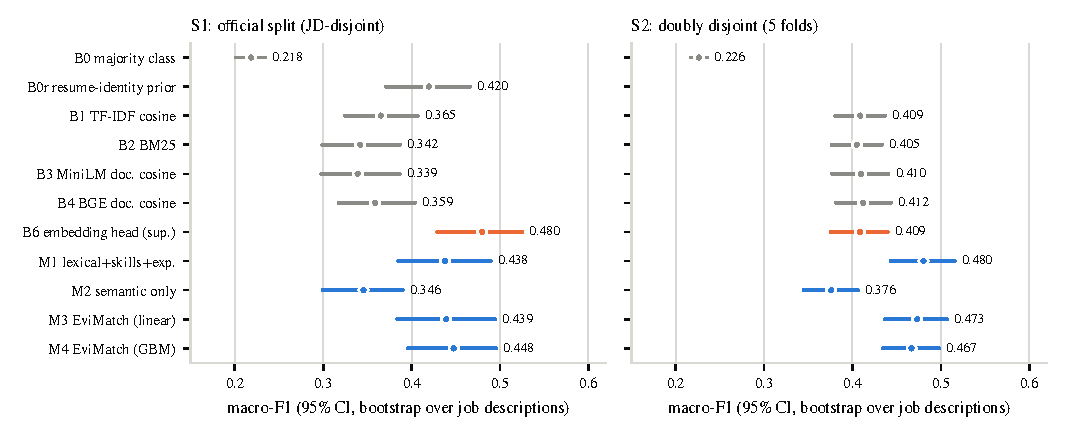
\includegraphics[width=\textwidth]{figures/fig_macro_f1.pdf}
\caption{Macro-F1 with 95\% intervals from bootstrap resampling of job descriptions. Gray: similarity
baselines and diagnostics; orange: supervised embedding head; blue: EviMatch variants.}
\label{fig:macrof1}
\end{figure*}

\begin{table}[t]
\caption{Per-class results of M3 on S2.}
\label{tab:perclass}
\centering\small
\begin{tabular}{lccc}
\toprule
Class & Precision & Recall & F1 \\
\midrule
No Fit & 0.731 & 0.606 & 0.663 \\
Potential Fit & 0.380 & 0.404 & 0.391 \\
Good Fit & 0.322 & 0.422 & 0.365 \\
\bottomrule
\end{tabular}
\end{table}

\begin{figure}[t]
\centering
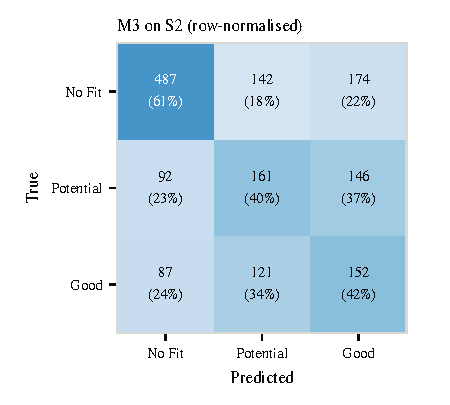
\includegraphics[width=0.78\columnwidth]{figures/fig_confusion.pdf}
\caption{Confusion matrix of M3 on S2 (counts and row percentages).}
\label{fig:cm}
\end{figure}

\subsection{Where the signal comes from}
Table~\ref{tab:ablation} and Fig.~\ref{fig:ablation} remove one feature group at a time. On S2,
removing the four \emph{experience} features costs 0.053 macro-F1 (CI $[-0.076,-0.029]$) and removing
\emph{skills} costs 0.032 ($[-0.056,-0.008]$). Removing the \emph{lexical} group changes nothing
($0.000$), and removing the \emph{semantic} group is, if anything, slightly positive ($+0.007$,
$[-0.015,+0.031]$). The four experience features alone reach 0.461, within noise of the full model
($-0.012$, $[-0.046,+0.026]$), although ranking quality then drops by 0.060 nDCG@10. In this benchmark the
labels appear to track how well a candidate's seniority and listed skills line up with the posting,
and the semantic coverage we expected to be central adds no significant accuracy. We still keep it,
because it supplies the sentence-level evidence that makes the score reviewable, but we do not claim that it
improves accuracy. Neither redaction ($0.000$ on S2, $+0.002$ on S1), the induced vocabulary, nor swapping
MiniLM for BGE-small ($+0.010$, $[-0.010,+0.033]$) changed accuracy measurably. The redaction result is a
lower bound on its cost because the benchmark's resumes are partly anonymised.

\begin{table}[t]
\caption{Ablations of M3 (macro-F1 and difference from the full model).}
\label{tab:ablation}
\centering\scriptsize
\resizebox{\columnwidth}{!}{\begin{tabular}{l rr rr}
\toprule
 & \multicolumn{2}{c}{S1} & \multicolumn{2}{c}{S2} \\
\cmidrule(lr){2-3}\cmidrule(lr){4-5}
Variant & macro-F1 & $\Delta$ & macro-F1 & $\Delta$ \\
\midrule
full & 0.439 & +0.000 & 0.473 & +0.000 \\
minus lexical & 0.434 & -0.005 & 0.473 & -0.000 \\
minus semantic & 0.438 & -0.001 & 0.480 & +0.007 \\
minus skills & 0.402 & -0.037 & 0.441 & -0.032 \\
minus experience & 0.394 & -0.045 & 0.420 & -0.053 \\
only lexical & 0.357 & -0.082 & 0.384 & -0.089 \\
only semantic & 0.346 & -0.094 & 0.376 & -0.097 \\
only skills & 0.405 & -0.034 & 0.417 & -0.056 \\
only experience & 0.417 & -0.022 & 0.461 & -0.012 \\
no redaction & 0.441 & +0.002 & 0.474 & +0.000 \\
no induced vocab & 0.435 & -0.004 & 0.468 & -0.006 \\
bge encoder & 0.426 & -0.013 & 0.483 & +0.010 \\
\bottomrule
\end{tabular}}
\end{table}

\begin{figure}[t]
\centering
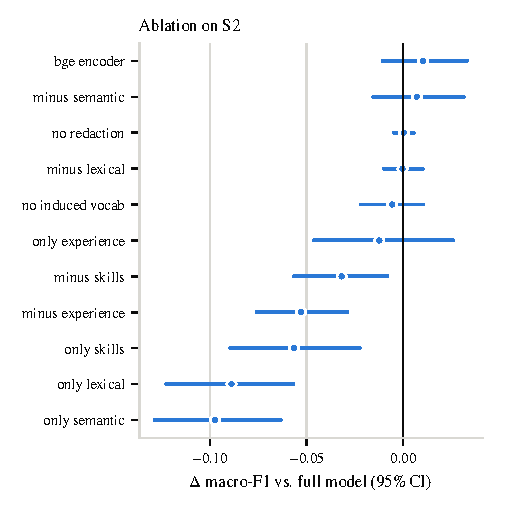
\includegraphics[width=\columnwidth]{figures/fig_ablation.pdf}
\caption{Change in macro-F1 on S2 when a component is removed or used alone.}
\label{fig:ablation}
\end{figure}

\subsection{Leakage}
Adding the seven single-document features to M3 (X1) raises S1 macro-F1 by $0.025$ (0.439 to 0.464;
paired $-0.024$, $[-0.056,+0.004]$) but changes S2 by only $+0.004$. The direction matches
the explanation that these features let a model recognise resumes, but with 71 test postings the S1
increase is not statistically significant, so we report it as consistent rather than conclusive. The
resume-identity prior and the S1/S2 behaviour of B6 are the stronger evidence.

\subsection{How much labelled data is needed?}
Fig.~\ref{fig:lc} trains on random subsets of training postings. With about 270 pairs M3 is already at
0.396 macro-F1, and it improves to 0.475 with about 5{,}100 pairs, whereas threshold baselines move from
0.384 to 0.406 and the embedding head from 0.374 to 0.409. Variation across runs is large (standard
deviation 0.02--0.06), so differences below about 0.03 at a single size should not be over-read.

\begin{figure}[t]
\centering
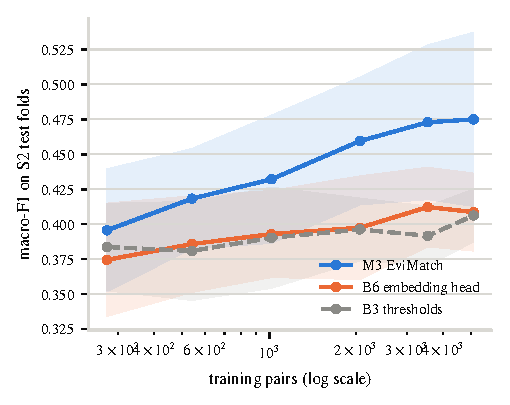
\includegraphics[width=\columnwidth]{figures/fig_learning_curve.pdf}
\caption{Macro-F1 on S2 test folds as a function of the number of training pairs
(mean of 15 runs, band $\pm1$ s.d.).}
\label{fig:lc}
\end{figure}

\subsection{Are the cited sentences faithful to the model?}
For 580 sampled test pairs we delete the sentences the explanation cites (the best sentences of the five
strongest met requirements plus the evidence of up to five skills, on average 5.1 sentences) and
re-score. The score falls by 7.7 points on average. Deleting the same number of words from randomly chosen
other sentences lowers it by 1.8 points. The difference of 5.9 points ($95\%$ CI $5.0$--$6.9$) holds for
86.7\% of pairs. Cited evidence is therefore not decorative. The test is a check against the model, not
a human study of whether reviewers find the explanations useful, which remains future work.
